\section{Results}
\label{section:results}

\subsection{Duty cycle}
Duty cycle describes the fractional time relationship of having the power supply active and not active. An example is a duty cycle of 50\%, meaning that the power supply is active 50\% of the time and not active the remaining 50\% of the time, this can be seen in Figure \ref{fig:duty_cycle}.

\begin{figure}[ht]
    \centering
    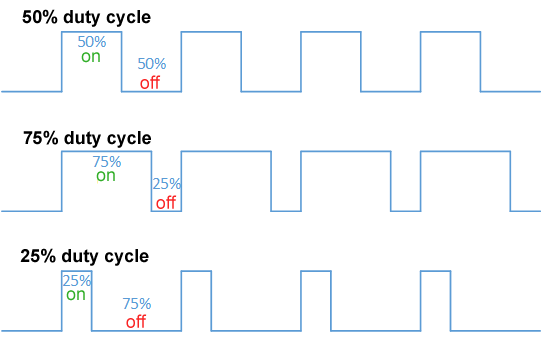
\includegraphics[width=0.9\columnwidth]{images/Duty_Cycle_Examples.png}
    \caption{Duty cycle. Original work of Thewrightstuff, https://commons.wikimedia.org/wiki/File:Duty\_Cycle\_Examples.png.}
    \label{fig:duty_cycle}
\end{figure}

\subsection{PWM (Pulse width modulation)}
PWM, or pulse width modulation, is a technique to control the average power to the load by switching (at a rate that wont significantly change the load) the power supply on and off to create a duty cycle. If we assume a system with a power supply of 5V, then with 50\% duty cycle, the load will act as if the power supply was 2.5V ($5*0.5=2.5$).

\subsection{ADC (Analog to digital converter)}
\begin{comment}
    An ADC, analog to digital converter, converts an analog signal to a digital signal which is important for most computer systems to be able to process the signal.
\end{comment}
The analog to digital converter on the TM4C129ENCPTD converts the analog voltages to digital discrete bits with a resolution of 12 bits. The resolution will convert the analog signal to be represented in bits between $0-2^{12}$. Without this conversion the microcontroller would not be able to process the analog signal since it only works in digital bits.

\subsection{UART (Universal asynchronous receiver-transmitter)}
UART, Universal asynchronous receiver-transmitter, is a hardware device which performs serial asynchronous communication. 


\subsection{Code 2.1}
The code for assignment 2.1 is controlled by sending the desired percentage over UART. The program checks if the value is in the interval $(0, 100)$, and if it is, the LED is controlled by PWM. The value is scaled to be in the range $[10, 990]$ where $10$ is the lowest brightness and $990$ the highest. If the value is either, $0$ or $100$ the LED should be turned on or off by using the LEDWrite API call.

\subsection{Code 2.2}
The code in 2.2 uses the potentiometer (joystick Y/vertical axis) rather than the UART to obtain the value for the duty cycle. First the 0 to 4095 value range of the potentiometer is mapped to a 0 to 100 range. The 0 to 100 range is then used as a percentage scale passed to the PWM to produce a duty cycle of 0 to 100\% to control the LED brightness/intesity. The PWM0\_BASE (which is on PF2 and uses PWM\_OUT\_2) was used and thus PWM\_GEN\_1 was also used \footnote{PWN\_GEN\_0 is connected to PWM 0 and 1, PWN\_GEN\_1 is connected to PWM 2 and 3, PWN\_GEN\_2 is connected to PWM 4 and 5, PWN\_GEN\_3 is connected to PWM 6 and 7}. It should be noted that joystick vertical (Y-axis) is on PE4 and uses channel 0, however it should be on PE3.



\begin{comment}
This section should present answers to all research questions.

It is normal to have only one results section, but you can create more sections if finding it more appropriate. You can also divide results into subsections. Perhaps you want to refer to some other section, for example (see Section \ref{section:method}). You can also place figures, you should always reference these in the text, see Figure \ref{fig:MDHlogga} for an example of a figure including subfigures. Remember that all figures should have a figure label explaining their content.


\begin{figure}[H]
    \centering
    \subfigure[MDH logo]{
    \label{fig:MDH1}
    
\includegraphics[width=.2\columnwidth]{MDHlogga}}
    \qquad
    \subfigure[MDH logo]{
    \label{fig:MDH2}
    
\includegraphics[width=.2\columnwidth]{MDHlogga}}
    \qquad
    \subfigure[MDH logo]{
    \label{fig:MDH3}
    
\includegraphics[width=.2\columnwidth]{MDHlogga}}
    \caption[Short text]{This is a example of multiple figures.}
    \label{fig:MDHlogga}
\end{figure}
\end{comment}